\documentclass[conference]{IEEEtran}
\usepackage{times}

% numbers option provides compact numerical references in the text. 
\usepackage[numbers]{natbib}
\usepackage{multicol}
\usepackage[bookmarks=true]{hyperref}
\usepackage{graphicx}
\usepackage{amsmath,amsfonts,amssymb}

\graphicspath{ {./graphics/} }

\pdfinfo{
   /Author (Mingyo Seo)
   /Title  (Robots: Our new overlords)
   /CreationDate (D:20101201120000)
   /Subject (Robots)
   /Keywords (Robots;Overlords)
}

\begin{document}

% paper title
\title{CS391L HW2: Independent Component Analysis}

% You will get a Paper-ID when submitting a pdf file to the conference system
\author{Mingyo Seo}

\author{\authorblockN{Mingyo Seo}
\authorblockA{
UT EID: ms84662\\
Email: mingyo@utexas.edu}}



\maketitle

\IEEEpeerreviewmaketitle

\begin{abstract}

In this assignment, an overview of Independent Component Analysis (ICA) is presented and is applied to separate a mixture of sounds. A set of 5 different sources were taken and mixed to obtain a 5 different "microphone" recordings. The ICA algorithm was applied to retrieve the individual sounds and the retrieval quality was examined.
\end{abstract}

\section{Introduction} % Introduce your problem and the overall plan for approaching your problem

The problem of seperating a certain signal from a mixture of multiple signals can be applied to many areas. The simplest example of this problem is the cocktail party problem where we have recordings from different microphones of the same mixture of conversations.
In this paper, in particular, we implemented an ICA to seperate voices from the mixture of conversations. 
We also studied the effects of parameters on the model's performance. The answers to the HW2 questions are included in the following sections.\begin{itemize}
\item Fig. \ref{fig:base}: Visualization of base source sounds
\item Fig. \ref{fig:mixed}: Visualization of mixed source sounds
\item Fig. \ref{fig:recovered}: Visualization of recovered source sounds
\item Fig. \ref{fig:batch_test}, \ref{fig:eta_test}: Correlation between orignal and recovered sounds
\end{itemize}



\section{Method}
\label{sec:method}

\subsection{Mixing matrix}
In this assignment, a test data set $U$ containing $5$ sound sources and $t$ number of samples is given. We aim to mix $n$ sources from the given sounds to generate a pseudo microphone output $X$ of $m$ recordings where $m\geq n$. To do this, we introduce a mixing matrix $A$, as
\begin{equation}
    X = AU
\end{equation}
Here, $X$ is a $m \times t$ matrix of the mixed sound signals.


\subsection{Independent Component Analysis}

Contrary to Principal Component Analysis which finds the primary features in the given dataset, the ICA method decomposes a mixture of signals into its individual sources. 

The goal of the ICA method is to find the un-mixing $n \times m$ matrix $W$, as
\begin{equation}
    WA = I.
\end{equation}
This yields of restoring the orignial signal $U$, as
\begin{equation}
    U = WX.
\end{equation}
We use the maximum likelihood estimate to find $\hat{W}$, an estimate of $W$, and the gradient descent to approximate it. These methods are described in the following subsections.


\subsection{Maximum Likelihood Estimation}
There are several methods available in literature that can be used to calculate the unmixing matrix $W$, \cite{} for example uses a SVD (singular value decomposition) methods to calculate the matrix W. There are advantages and disadvantages to the available approaches. For example, the SVD approach involves calculation of the Eigenvalues of $XX^T$ which may be slow if the number of microphone inputs (m) is large.
The Maximum Likelihood Estimate (MLE) of $W$ is calculated by maximizing the parameters of W to match the mixed data X. To do this, the following definition is used for the likelihood of the mixture X:

\begin{equation}
    p(x=X) = p_x(X) = p_u(U)\cdot|W| = \prod_{i=1}p_i(u_i)|W|    
\end{equation}

where, $p_u(U)$ is the probability density function of the independent source signals, and $p_i(u_i)$ is the probability density of the $i_{th}$ source component\\

Since we have $t$ samples of all mixtures in X, we can calculate $P_x(X)$ as:


\begin{equation}
    L(W) = \prod_{j=1}^t\prod_{i=1}^np_i(w_i^Tx_j)|W|
    \label{eq:likelihood def}
\end{equation}
where, $x_j$ is the $j^{th}$ column of X.\\
Thus our goal is to maximize $L(W)$ over all $W$, i.e.:
\begin{equation}
    \max_{W\epsilon R^{(n,m)}} L(W)
    \label{eq:optimality-eqn}
\end{equation}
Given that the probability density function is always positive, we can maximize $L(W)$ by maximizing the log likelihood function. The reason for maximizing log likelihood is because, taking log of $L(W)$ changes the product terms in $W$ into summation terms, i.e.:

\begin{eqnarray}
    \ln{(L(W))} =& \sum_{j=1}^t\sum_{i=1}^n\ln{(p_i(w_i^Tx_j)|W|)}&\\
     =& \sum_{j=1}^t\sum_{i=1}^n\ln{(p_i(w_i^Tx_j)}& + \sum_{i=1}^n\ln(|W|)\\
     \therefore \ln{(L(W))} =& \sum_{j=1}^t\sum_{i=1}^n\ln{(p_i(w_i^Tx_j)}& + t\ln{(|W|)}
     \label{eq:simplified loglike}
\end{eqnarray}
We can simplify equation \ref{eq:simplified loglike} further as:
\begin{equation}
    \frac{1}{t}\ln{(L(W))} = E\left[\sum_{i=1}^n\ln{(p_i(w_i^Tx_j))}\right] + \ln{(|W|)}
    \label{eq:log-like-Exp}
\end{equation}
where E[] is the expectation/mean observation. \\
Here we introduce the concept of the cumulative density function (cdf). The cumulative density function $g(X)$ is the integral of the pdf, and gives the net probability of the function having a value below X. Thus the pdf $p(X)$ is simply the derivative of $g(X)$. Thus equation \ref{eq:log-like-Exp} becomes,\\
\begin{equation}
    \frac{1}{t}\ln{(L(W))} = E\left[\ln{(g'(WX)}\right] + \ln{(|W|)}
    \label{eq:log-like-Exp-cdf} 
\end{equation}

There are many algorithms that are available for maximizing the the log-likelihood function. Gradient descent algorithm is a popular approach to maximize $L(W)$. Since we maximize with respect to W, the gradient is taken accordingly, i.e.:
\begin{equation}
\label{eq:grad}
\begin{aligned}
    \frac{1}{t}\frac{\partial}{\partial W}\ln(L(W)) \\
    = E\left[\frac{\partial}{\partial W}(\ln{(g'(WX)})X^T\right] + \frac{\partial}{\partial W}\ln{(|W|)} \\
    = E\left[\frac{\partial}{\partial W}(\ln{(g'(WX)})X^T\right] + \left[W^T\right]^{-1}
\end{aligned}
\end{equation}


\subsection{Gradient Descent}
The gradient descent method is an iterative algorithm to find a function's minimum or maximum points. If the convex function is convex, the gradient descent converges to the global extremums. Otherwise, it converges to the local extremums. Proving the convexity of the log likelihood $L(W)$ is beyond the scope of this report, so it is not described in this report.

Gradient descent starts at an initial point $\hat{W}_0$ and updates it by moving to next points recursively along the gradient computed at previous points. To formulate the gradient descent method in terms of $W$, the estimate $\hat{W}_{k}$ of the $W$ matrix after the $k^{th}$ iteration is given as, 
\begin{equation}
\begin{aligned}
    \hat{W}_{k+1} &= \hat{W}_k + \eta\cdot\left(\frac{1}{t}\frac{\partial}{\partial W}\ln(L(W))\right)_{W=\hat{W}_k}\\
     &= \hat{W}_k + \eta\cdot\Delta W,
\end{aligned}
\end{equation}
where $\eta$ is the {\it learning rate} of the gradient descent.
Here, the initial point $\hat{W}_0$ is given randomly, and $\eta$ should be adjusted to acheive convergence.

From Equation \ref{eq:grad}, the gradient term contains $\left[W^T\right]^{-1}$ which requires expensive computation for the inverse operation. 
Thus, we process the interation by multiplying it with $W^TW$, which preservers the convergence to the optimum, and avoids the inverse operation, as
\begin{equation}
\begin{aligned}
    \Delta W
    &= \frac{1}{t}\frac{\partial}{\partial W}\ln(L(W)) W^T \\
    &= E\left[\frac{\partial}{\partial W}(\ln{(g'(WX)})X^T\right] W^TW + \left[W^T\right]^{-1} W^TW \\
    &= \left(E\left[\left(\frac{\partial}{\partial W}(\ln{(g'(WX)})\right)(WX)^T\right] W + W\right)_{W=\hat{W}_k}.
    \label{eq:delta W simplified}
\end{aligned}
\end{equation}
The above formulation does not affect the  optimality of equation \ref{eq:optimality-eqn}. Decription for this is omitted for brevity of this report, and we encourage to refer the class notes.

To facilitate the gradient descent algorithm, we need to choose a globally differentiable $cdf$. In particular, we used the following $cdf$,
\begin{equation}
    g(WX) = \frac{1}{1+e^{-WX}}.
\end{equation}
It is differentiable for all $WX$ and is bounded in $\left[0,1 \right]$. The derivative of $g$ is given as
\begin{equation}
\label{eq:deriv}
    g'(WX) = g(WX)(1-g(WX)).
\end{equation}
Inserting Equation \ref{eq:deriv} into Equation \ref{eq:delta W simplified} yields
\begin{equation}
    \Delta W = \left(\left(E\left[(1-2g(WX))(WX)^T\right] + I \right)W\right)_{W=\hat{W}_k}.
\end{equation}

To summarize the processes described above, the algorithm is implemented as:
\begin{enumerate}
    \item Start with an intial point $\hat{W}_0$.  
    \item Compute matrix $Z_k = g(\hat{W}_kX)$
    \item Compute $\Delta W = \left(E\left[(1-2Z_k)(\hat{W}_kX)^T\right] + I \right)\hat{W}_k$.
    \item Update the estimation as $\hat{W}_{k+1} = \hat{W}_k + \eta\cdot\Delta W$
    \item Return to Step 2 and repeat the processes until it reaches the maximum iteration.
\end{enumerate}


\section{Results} % Describe the methods you intend to apply to solve the given problem

The classifier model of PCA and KNN methods described in Section \ref{sec:method} is implemented python scripts (3.8.5).

\subsection{Model Training}
We trained with the first 1000 samples of the training set, and the result eigenvalues are presented in descending order in Fig. \ref{fig:eig_vals}.
The eigenvectors of the principal components are presented in Fig. \ref{fig:eig_vecs}.
For evaluation of the model, we chose the principal component $M=15$ and KNN size $K=5$, and the model achieves an accuracy of 84.35 \%.


\subsection{Batch size}

The plot of accuracy of with different number of trainign samples is presented in Fig. \ref{fig:sample_test}.
In the experiment, we used $M=24$, and $K=5$.
There is trade-off in using a larger training sample size: the accuracy increases as a training sample size increases but computation time also increases linearly.

\begin{figure}[!t]
	\centering
	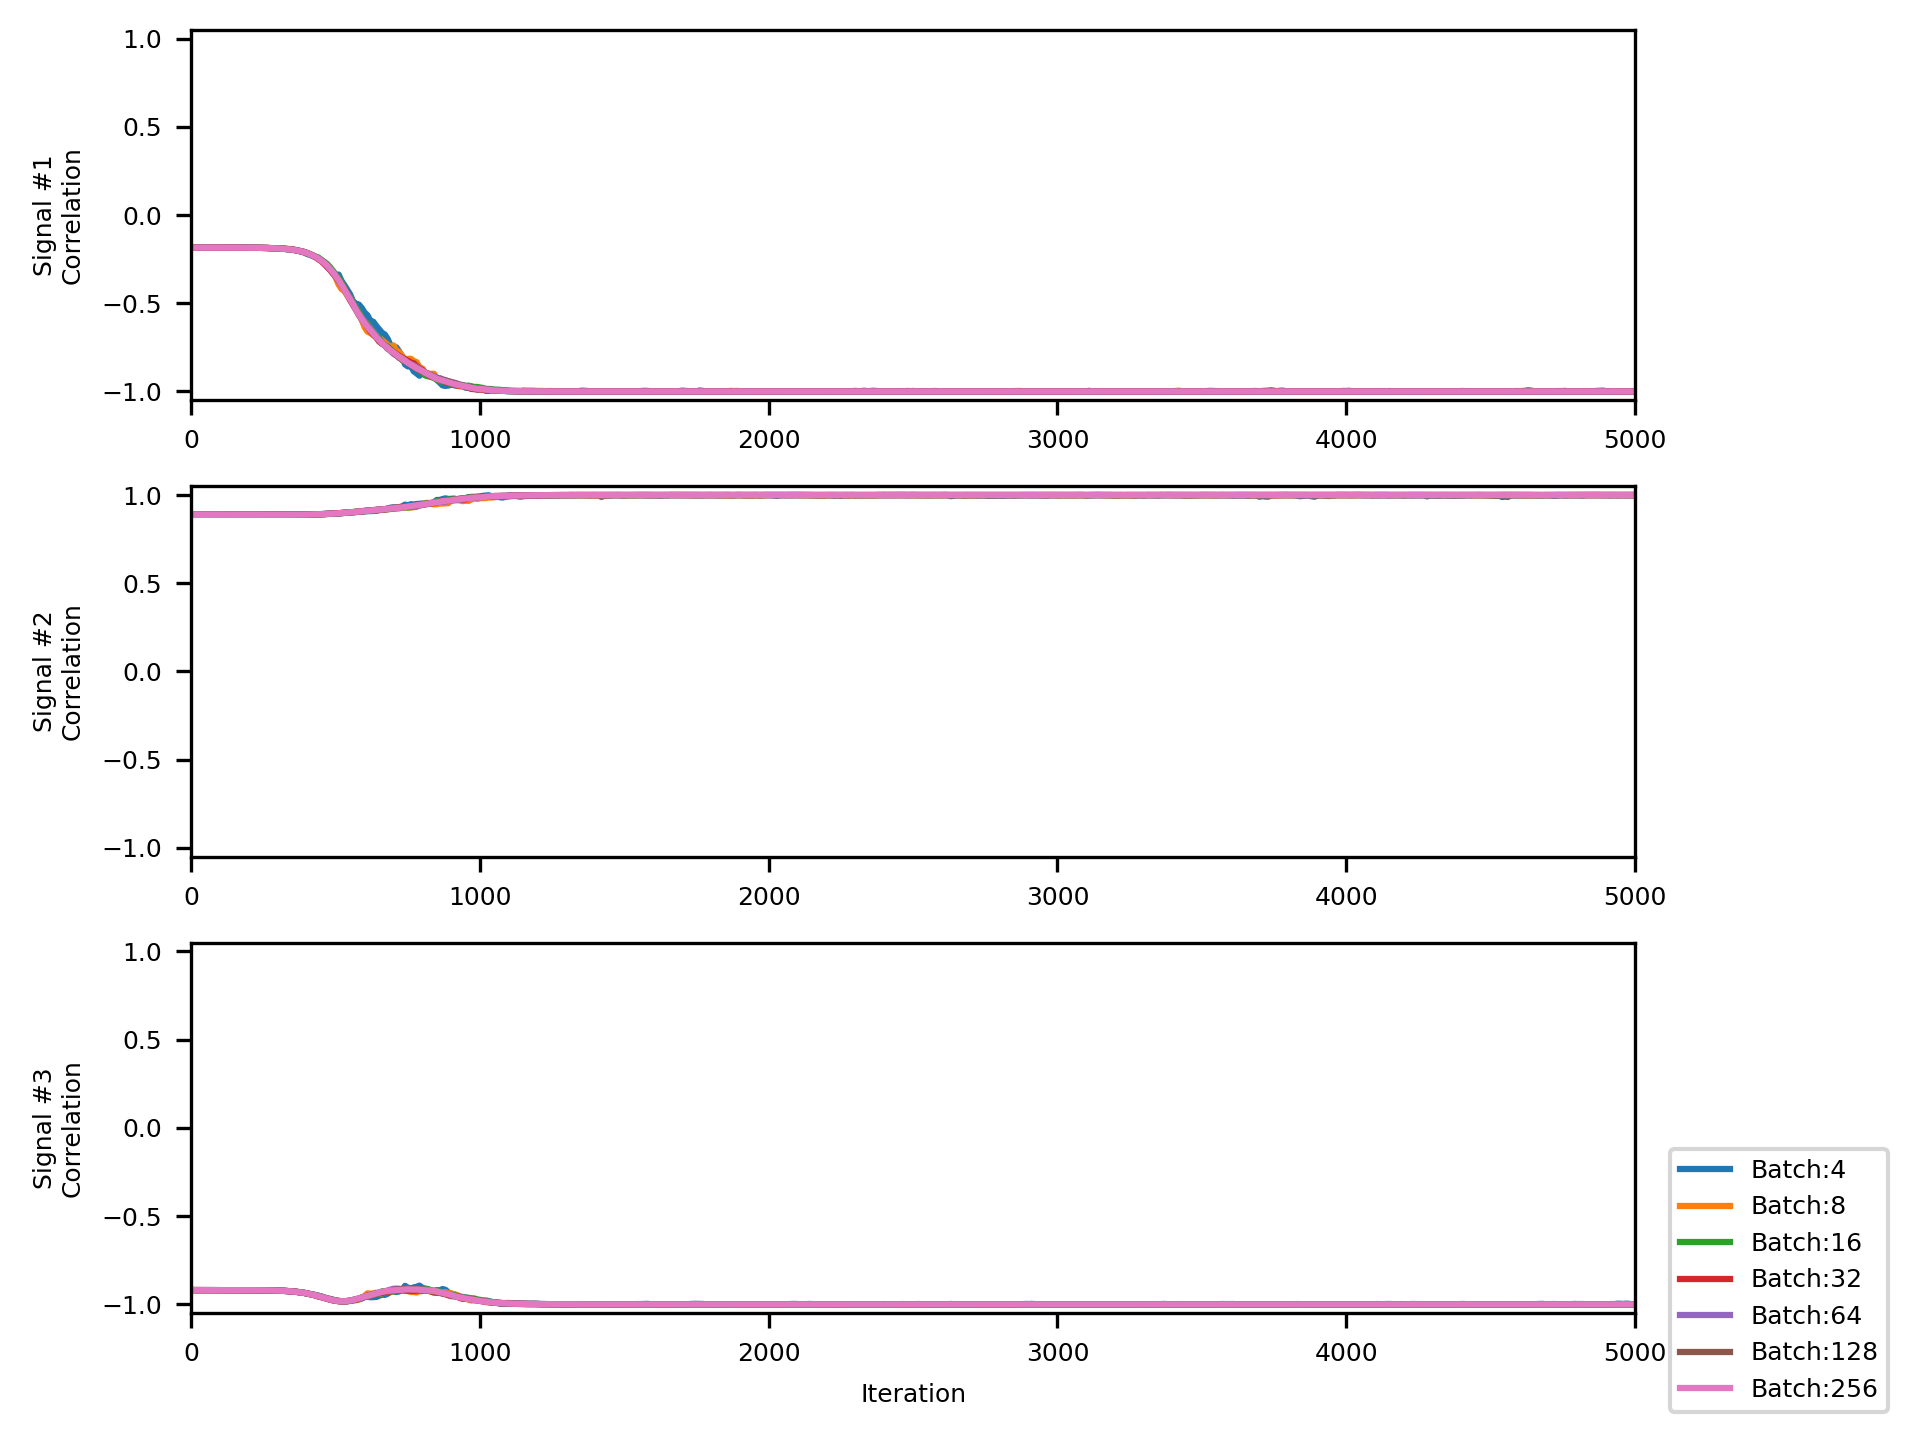
\includegraphics[width=3.6in]{source3/batch_test.png}	
	\caption{Accuracy and computation time changes on training sample size: training sample sizes are chosen in [300, 500, 1000, 5000, 10000, 30000, 60000].}
	\label{fig:batch_test}
\end{figure}


\subsection{Learning rate}

The plot of the accuracy of with different KNNs is presented in Fig. \ref{fig:knn_test}.
In the experiment, we used $M=24$, and 1000 training samples.
The accuracy for inferring worsens as KNN size increases, the computation time does not change much.

\begin{figure}[!t]
	\centering
	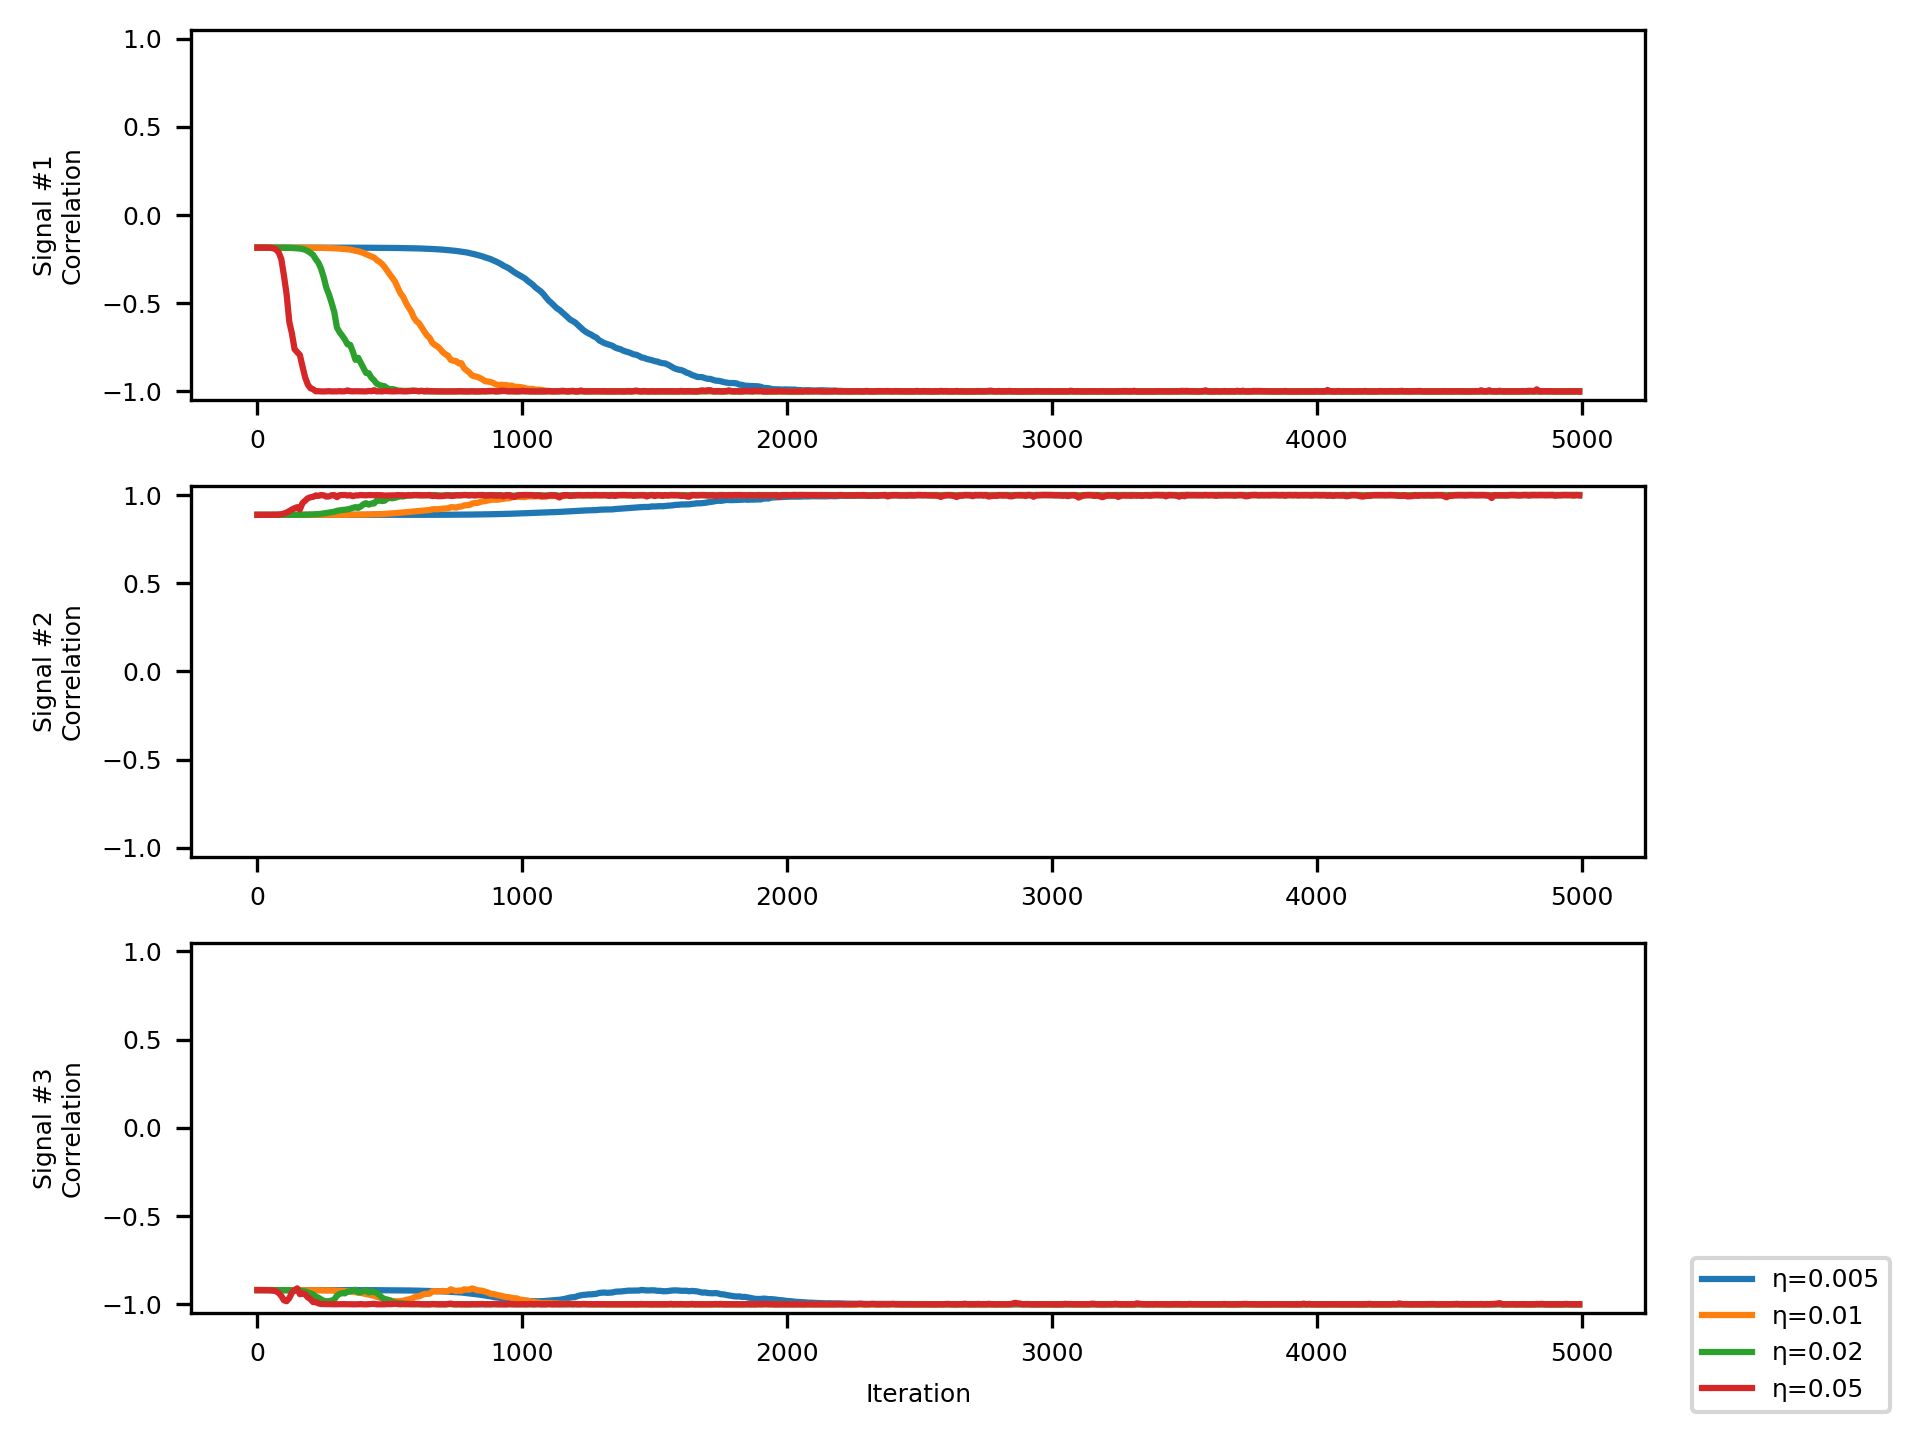
\includegraphics[width=3.6in]{source3/eta_test.png}	
	\caption{Accuracy and computation time changes on KNN sizes: KNN sizes are chosen in [1, 3, 5, 10, 25].}
	\label{fig:eta_test}
\end{figure}



\section{Summary} %Intermediate/Preliminary Results: State and evaluate your results upeto the milestone
The classifier method of PCA and KNN for classifying digit character images are implemented in the assignment. For evaluation, we used the MNIST dataset. From the results of the experiments, a smaller KNN size benefits the accuracy. However, for the PCA size, the accuracy peaked at $M=50$, This implies that enough number of feature is required for estimation but too many features distract the proper labels, which worsen the accuracy. On the other hand, a larger training size yields higher accuracy but also requires higher computation power.



%\section*{Acknowledgments}

%% Use plainnat to work nicely with natbib. 

\bibliographystyle{plainnat}
\bibliography{references}

\end{document}


